\documentclass{article}

% Matemática y símbolos
\usepackage{amsmath}
\usepackage{amssymb}

% Márgenes y geometría de la página
\usepackage{geometry}
\geometry{a4paper, margin=1in, bottom=2cm}

% Colores y cajas
\usepackage{xcolor}
\usepackage{mdframed}

% Gráficos y diagramas
\usepackage{tikz}
\usetikzlibrary{positioning}  % Para posicionamiento relativo en TikZ

% Tablas elegantes y columnas personalizadas
\usepackage{booktabs}
\usepackage{array}
\usepackage{float}

% Imágenes
\usepackage{graphicx}

% Estilo de párrafo
\usepackage{parskip}

% Idioma
\usepackage[spanish]{babel}
\usepackage[utf8]{inputenc}  % Si no usas UTF-8 nativo

% Captions
\usepackage{caption}

% Información del documento
\title{Guía de Problemas: PERT/CPM}
\author{Ricardo Largaespada}
\date{04 de abril 2025}

% Entorno personalizado para problemas
\newmdenv[
  backgroundcolor=blue!5,
  linecolor=blue,
  linewidth=1pt,
  roundcorner=5pt,
  skipabove=\baselineskip,
  skipbelow=\baselineskip
]{problem}


\begin{document}

\maketitle

\begin{problem}
\textbf{Problema 1 | CPM}\\
La siguiente tabla presenta las actividades necesarias para adquirir un automóvil nuevo. En este caso, la red debe construirse utilizando una representación con \textbf{actividad en el arco} (AOA), donde los nodos representan eventos y las actividades están en los arcos.

\medskip

\textbf{Solicitudes:}
\begin{enumerate}
    \item Construya la red del proyecto utilizando el método de actividad en el arco.
    \item Determine la \textbf{duración total del proyecto}.
\end{enumerate}

\begin{table}[H]
\centering
\begin{tabular}{l p{6cm} c c}
\toprule
\textbf{Actividad} & \textbf{Descripción} & \textbf{Predecesora(s)} & \textbf{Duración (días)} \\
\midrule
A & Realizar estudio de factibilidad & --- & 3 \\
\hline
B & Encontrar un comprador potencial para el automóvil actual & A & 14 \\
\hline
C & Poner en lista los posibles modelos & A & 1 \\
\hline
D & Entrevistarse con el mecánico & C & 3 \\
\hline
E & Reunir publicidad del concesionario & C & 1 \\
\hline
F & Compilar los datos pertinentes & C & 2 \\
\hline
G & Completar los datos pertinentes & D, E, F & 1 \\
\hline
H & Escoger tres modelos & G & 1 \\
\hline
I & Realizar prueba de manejo de las tres opciones & H & 3 \\
\hline
J & Conseguir garantía y datos de financiamiento & H & 2 \\
\hline
K & Escoger un automóvil & I, J & 2 \\
\hline
L & Elegir el concesionario & K & 2 \\
\hline
M & Buscar el color y opciones deseadas & L & 4 \\
\hline
N & Realizar prueba de manejo del modelo una vez más & L & 1 \\
\hline
O & Comprar el automóvil nuevo & B, M, N & 3 \\
\bottomrule
\end{tabular}
\caption{Actividades para adquirir un automóvil nuevo}
\end{table}

\end{problem}

\newpage

\begin{problem}
\textbf{Problema 2 | CPM}\\
En la tabla siguiente se presentan las actividades relacionadas con el servicio coral a la luz de las velas. Se requiere construir la red empleando una representación de \textbf{actividad en el arco} (AOA), con nodos que simbolizan eventos y arcos que representan las actividades.

\medskip

\textbf{Solicitudes:}
\begin{enumerate}
    \item Construya la red del proyecto utilizando el método de actividad en el arco.
    \item Determine la \textbf{duración total del proyecto}.
\end{enumerate}

\begin{table}[H]
\centering
\begin{tabular}{l p{6cm} c c}
\toprule
\textbf{Actividad} & \textbf{Descripción} & \textbf{Predecesora(s)} & \textbf{Duración (días)} \\
\midrule
A & Seleccionar la música & --- & 2 \\
\hline
B & Aprenderse la música & A & 14 \\
\hline
C & Sacar copias y comprar libros & A & 14 \\
\hline
D & Audiciones & B, C & 3 \\
\hline
E & Ensayos & D & 70 \\
\hline
F & Rentar candelabros & D & 14 \\
\hline
G & Decorar los candelabros & F & 1 \\
\hline
H & Instalar las decoraciones & F & 1 \\
\hline
I & Pedir atuendos para el coro & D & 7 \\
\hline
J & Verificar el sistema de sonido & D & 7 \\
\hline
K & Seleccionar las pistas de música & J & 14 \\
\hline
L & Instalar el sistema de sonido & K & 1 \\
\hline
M & Ensayo final & E, G, L & 1 \\
\hline
N & Reunión del coro & H, I, M & 1 \\
\hline
O & Programa final & I, N & 1 \\
\bottomrule
\end{tabular}
\caption{Actividades para organizar el programa del coro}
\end{table}

\end{problem}
\newpage
\begin{problem}
\textbf{Problema 3 | PERT}

El grupo de desarrollo de producto en Landon Corporation ha trabajado en un nuevo producto de software que tiene el potencial de capturar un gran segmento del mercado. A través de fuentes externas, la gerencia de Landon se dio cuenta que el competidor trabaja en un producto similar. Por consiguiente, la alta gerencia de Landon incrementó su presión en el grupo de desarrollo de productos. El líder del grupo recurrió al procedimiento PERT/CPM para programar las actividades restantes antes de que el nuevo producto pueda ser llevado al mercado. La red del proyecto es la siguiente:

\textbf{Red del Proyecto}

\begin{center}
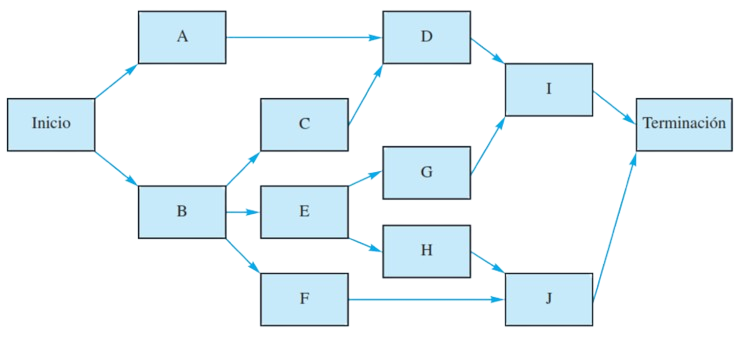
\includegraphics[scale=0.5]{images/10-problema2.png}
\end{center}

\textbf{Tiempos estimados de las actividades}
\begin{center}
\begin{tabular}{|l|c|c|c|}
\hline
\textbf{Actividad} & \textbf{Optimista (O)} & \textbf{Más probable (M)} & \textbf{Pesimista (P)} \\
\hline
A & 3.0 & 4.0 & 5.0 \\
B & 3.0 & 3.5 & 7.0 \\
C & 4.0 & 5.0 & 6.0 \\
D & 2.0 & 3.0 & 4.0 \\
E & 6.0 & 10.0 & 14.0 \\
F & 7.5 & 8.5 & 12.5 \\
G & 4.5 & 6.0 & 7.5 \\
H & 5.0 & 6.0 & 13.0 \\
I & 2.0 & 2.5 & 6.0 \\
J & 4.0 & 5.0 & 6.0 \\
\hline
\end{tabular}
\end{center}
\textbf{Tarea}

En las siguientes secciones se calcularán:

\begin{itemize}
  \item Desarrolle un programa de actividades para este proyecto e identifique las actividades de ruta crítica.
\item ¿Cuál es la probabilidad de que el proyecto se complete de modo que Landon Corporation pueda lanzar el nuevo producto dentro de 25 semanas? ¿Dentro de 30 semanas?
\end{itemize}
\end{problem}

\newpage
\begin{problem}
\textbf{Problema 4 | PERT}

El gerente del Oak Hills Swimming Club planea un programa para el equipo de natación del club. La primera práctica del equipo se programó para el 1 de mayo. Las actividades, sus predecesoras inmediatas, y las estimaciones de los tiempos de actividad (en semanas) son las siguientes: 

\begin{center}
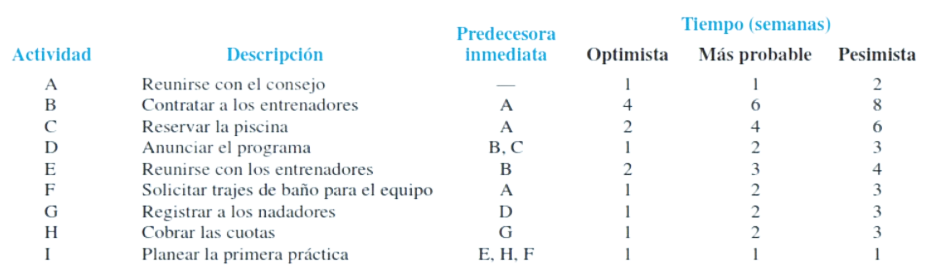
\includegraphics[width=\linewidth]{images/10-problema4.png}
\end{center}

En las siguientes secciones se calcularán:

\begin{itemize}
    \item Trace una red del proyecto.
    \item Desarrolle un programa de actividades.
    \item ¿Cuáles son las actividades críticas, y cuál es el tiempo de terminación del proyecto?
    \item Si el gerente del club planea iniciar el proyecto el 1 de febrero, ¿cuál es la probabilidad de que el programa de natación estará lista para la fecha programada del 1 de mayo (13 semanas)? ¿El gerente deberá comenzar a planear el programa de natación antes del 1 de febrero? 
\end{itemize}
\end{problem}

\end{document}
